
\section{Support d'étude \label{ccs_mp_2022_sec_1}}
%I.A - 
\subsection{Contexte \label{ccs_mp_2022_sec_1A}}
\ifprof
\else
L'obligation réglementaire de présence d'appui-têtes dans les voitures a contribué à une meilleure protection des conducteurs et des passagers en limitant les traumatismes dus au «coup du lapin » (figure \ref{ccs_mp_2022_fig_01}). Ce phénomène correspond à un mouvement brusque de flexion-extension de la tête par rapport au buste. Il peut être causé en voiture, lors de chocs à basse vitesse par exemple, ou dans des situations d'embouteillage. Aucune lésion n'est visible en imagerie médicale, cependant les victimes de ce traumatisme cervical souffrent de douleurs handicapantes sur le long terme.\\

\begin{figure}[!h]
\centering
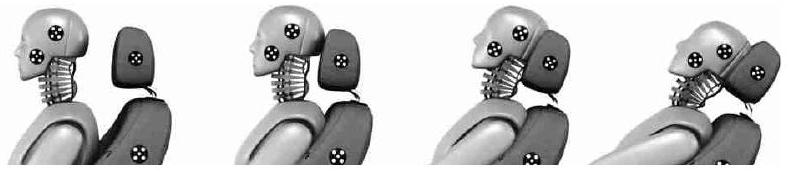
\includegraphics[width=\textwidth]{2025_07_06_ec63d2f3afc18cdeeb83g-01}

%Figure 1 
\caption{Réduction du phénomène du «~coup du lapin~» par l'usage d'un appui-tête (Référence : R.T. Shone) \label{ccs_mp_2022_fig_01}}
\end{figure}

Les crash-tests automobiles réalisés actuellement, sont effectués, entre autres, grâce à des mannequins de choc instrumentés représentatifs de différentes catégories de morphologie (par exemple, le mannequin représentant $50 \%$ des tests, correspond à un homme mesurant $1,75 \mathrm{~m}$ et pesant 80 kg ). L'étude de la diversité morphologique n'est cependant pas complète. De plus, la contribution musculaire de l'humain qui réagit au choc ne peut pas être étudiée. Mais surtout, les systèmes expérimentaux de crash-tests déjà disponibles ne sont pas représentatifs du phénomène de «coup du lapin» en termes d'accélérations et d'énergie dissipée lors du choc.\\
L'étude proposée porte sur la conception d'un dispositif expérimental, appelé Sled, ainsi que son modèle numérique, qui serviront, dans le cadre de travaux de recherche, à mieux comprendre les phénomènes liés au «~coup du lapin » et ainsi à adapter à terme les moyens de prévention et de protection des individus en fonction des morphologies. La conception s'articule en 3 étapes.

\begin{itemize}
  \item Première étape : conception d'un Sled $0,3 g$
\end{itemize}

Afin de comprendre les traumatismes causés par le phénomène de «coup du lapin », il est nécessaire, de développer un dispositif expérimental particulier, permettant de générer des niveaux d'énergie faibles et non lésionnels à un volontaire. Ces faibles niveaux d'énergie correspondent à des accélérations et décélérations fixées à $\pm 0,3 g$ pendant une durée de 1 seconde chacune.

\begin{itemize}
  \item Deuxième étape : élaboration de modèles
\end{itemize}

Ces données, recueillies sur des personnes volontaires, serviront à enrichir une base de données et permettront de développer des modèles de comportement à ce niveau d'énergie, mais aussi à des niveaux d'énergie réels (accélération/décélération de $\pm 1 g$ pendant 1 seconde).

\begin{itemize}
  \item Troisième étape : conception d'un Sled $1 g$
\end{itemize}

Un second dispositif expérimental sera ensuite construit. Avec des accélérations de $\pm 1 g$, les expérimentations ne pourront être conduites qu'avec des mannequins de chocs. Ce second dispositif, plus représentatif en ce qui concerne les niveaux d'accélération, servira alors à affiner les modélisations numériques.

La modélisation biomécanique des individus ainsi que les réactions musculaires des volontaires ne seront pas étudiées ici. Le sujet portera exclusivement sur les deux premières étapes.
Le principe retenu par les ingénieurs du bureau d'études pour concevoir le Sled (figure \ref{ccs_mp_2022_fig_02}) est inspiré des crashtests réalisés dans le domaine automobile :

\begin{itemize}
  \item une plateforme est animée d'un mouvement de translation horizontale par rapport au bâti ;
  \item un passager (volontaire ou mannequin) peut prendre place sur cette plateforme via un siège ;
  \item un dispositif de mise en mouvement permet d'atteindre les accélérations et décélérations attendues.
\end{itemize}


\begin{figure}[!h]
\centering
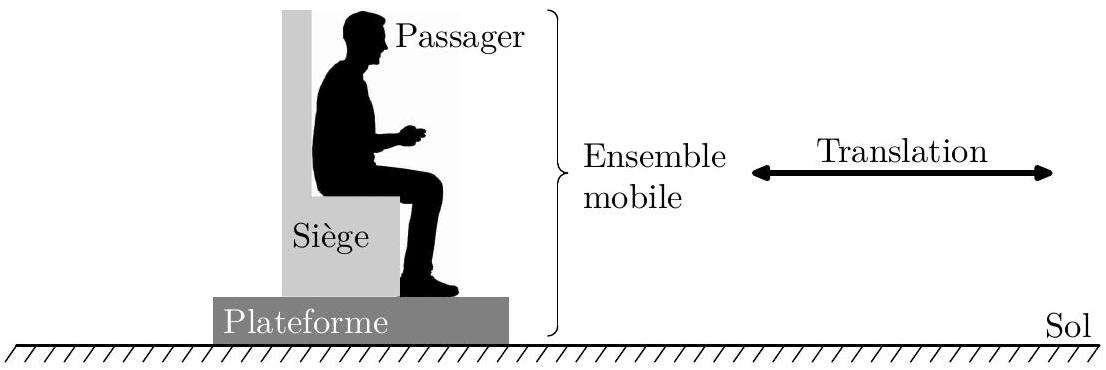
\includegraphics[width=\textwidth]{2025_07_06_ec63d2f3afc18cdeeb83g-02(1)}

%Figure 2 
\caption{Principe retenu pour la conception du Sled \label{ccs_mp_2022_fig_02}}
\end{figure}
\fi

%I.B - 
\subsection{Diagramme partiel des exigences du Sled pour les versions $0,3 g$ et $1 g$ \label{ccs_mp_2022_sec_1B}}
\ifprof
\else
Afin que les accélérations et les vitesses générées soient représentatives du phénomène de "coup du lapin », le Sled doit satisfaire les exigences définies figure \ref{ccs_mp_2022_fig_A} du document réponse.
\fi

